\section{Overall description}

\subsection{Product perspective}
	
	\todo{description}
	\begin{figure}[h]
			\centering
			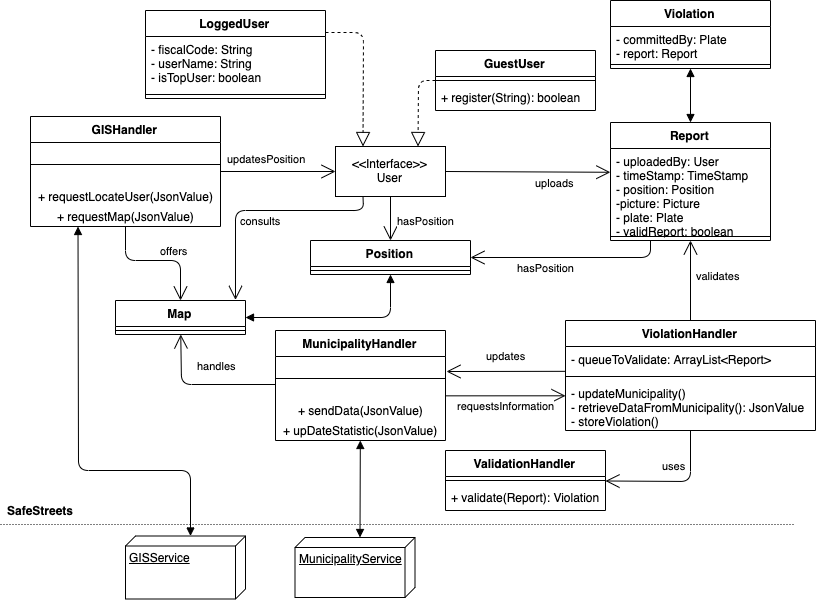
\includegraphics[width=300pt, height=200pt]{uml}
			\caption{
				\label{fig:systemInterfaces} 
				Class Diagram
			}
		\end{figure}

	\subsubsection{System interfaces}
	\label{sec:systemInterfaces}
		The system we are to develop will have some external interfaces (represented in \autoref{fig:systemInterfaces}) to accomplish the \hyperref[sec:goals]{goals stated before}.
		\begin{figure}[h]
			\centering
			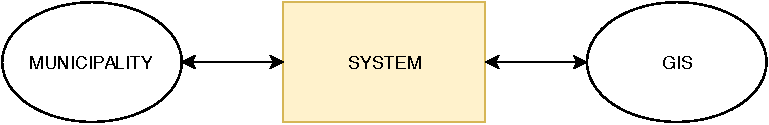
\includegraphics[width=300pt, height=50pt]{system_blocks}
			\caption{
				\label{fig:systemInterfaces} 
				Overview of system interfaces
			}
		\end{figure}
	\paragraph{Municipality}
	The system will interact with municipalities. Our system will retrieve the information about the accidents that occur on the territory of the municipality and cross this information with its own data to identify potentially unsafe areas. It will also retrieve the information about issued tickets from the municipalities to build statistics, for example about the most egregious offenders, or the effectiveness of the SafeStreets initiative (e.g., by looking for trends in the issuing of tickets).
	
	 In addition, our system will expose via a \emph{restricted access API} the stored information about the violations to the municipalities, so that the local authorities can generate traffic tickets from it, and receive suggestions for possible interventions (e.g., add a barrier between the bike lane and the part of the road for motorized vehicles to prevent unsafe parking). 
	 
	\paragraph{Map} Highlighted streets (or areas) with the highest frequency of violations, and unsafe areas are displayed to all users on an up-to-date map which relies on an external GIS.

\subsubsection{User interfaces}		
\paragraph{Guest user}
	Using the interfaces of the system users can:
	\begin{enumerate}
		\item Register to the system or request an account for a specific municipality
		\item Log-in to the system
	\end{enumerate}
\paragraph{Logged User}
	Using the interfaces of the system users can:
	\begin{enumerate}
		\item Submit a violation with all the required and optional metadata
		\item View a map through an external GIS with highlighted streets (or areas) with the highest frequency of violations
		\item View statistics on vehicles that commit the most violations, the most egregious offenders, or the effectiveness of the SafeStreets initiative.
			\todo{Siamo sicuri di voler fare che tutti gli utenti possono vedere queste staitistiche?}
		\item View and edit personal information
	\end{enumerate}
	
\subsubsection{Hardware interfaces}
	The only hardware interfaces with which the system cooperates are the smartphones of the users and the hardware that supports the system that offers municipality's service.
	
\subsubsection{Software interfaces}
	In order to reach the goals highlighted in the \hyperref[sec:goals]{goals section} the system need to interface with:
	\begin{enumerate}
		\item Databases and DBMSs, clearly required in order to store data about users, violations, safe/unsafe areas etc.
		\item The software offered by the municipality, required in order to exchange data with its services
		\item The map API offered by the GIS
	\end{enumerate}
	
\subsubsection{Communication interfaces}
	We want to ensure the encryption of data shared with our system. This involves recording of metadata information as well as issues of access control and security for all the handling digital chain of custody.
	
\subsection{Product functions}
\paragraph{Violation upload procedure} 
Provide logged users with the possibility to notify authorities when traffic violations occur and, in particular, parking violations. The application allows users to send pictures of violations, including their date, time, and position, to authorities. 
SafeStreets then stores the information provided, completing it with suitable meta-­data. In particular, when it receives a picture, it runs an algorithm to read the license plate number (the user can help with the recognition) and it stores the retrieved information with the violation, including also the type of the violation (submitted by the user) and the name of the street where the violation occurred.

\paragraph{Retrieve data from municipality}
Retrieve the information about the accidents that occur on the territory using the service offered by the municipalities and cross these data with SafeStreets data, to identify potentially unsafe areas. This will also allow the system to understand which violations are more likely to cause accidents in a particular zone and elaborate suggestions on possible interventions, later communicated to the municipality via a \emph{restricted access API} provided to them.

\paragraph{Show information and statistics}
The application allows logged users to mine the information that has been received, highlighting the streets (or the areas) with the highest frequency of violations, considered unsafe areas, or the vehicles that commit the most violations. In addition, statistics about issued tickets, for example about the most egregious offenders, or the effectiveness of the SafeStreets initiative, are shown to the user if requested. 

\paragraph{Restricted access API}
The system will expose via a \emph{restricted access API} the stored information about the violations to the municipalities, so that the local authorities can generate traffic tickets from it and receive suggestions for possible interventions to carry out (e.g., add a barrier between the bike lane and the part of the road for motorised vehicles to prevent unsafe parking), in order to decrease the risk of those areas, so increasing their safety. 



\subsection{User Characteristics}
	Users can use our system when they notice a violation and want to communicate it to the authorities.\\
 	Necessary conditions for the user in order to use the system are:
 	\begin{itemize}
 		\item He must have a smartphone with a working connection to the internet and he must be able to properly use it
 		\item He must be in the age of majority
 		\item He must be able to identify a violation and its type
 	\end{itemize}
 	The user agrees to these conditions during the registration to the system.
 	
\subsection{Constraints}
	We assume that these constraints are always met:
	\begin{enumerate}[label=\textbf{C\arabic*}]
		\item GPS position is supposed to be accurate (max error $\pm5$m)
		\item The quality of the picture is sufficient to recognise the plate number (min resolution 320x240)
		\item Internet connection must be strong enough to allow the upload of the picture in a reasonable amount of time (supported technologies are 3G, 4G and 5G due to the performance requirement)
	\end{enumerate}
	
\subsection{Assumptions}
	We assume that these assumptions hold true in the domain of our system 
	\begin{enumerate}[label=\textbf{	DA\arabic*}]
		\item GPS position of all users is always obtainable
		\item Internet connection always works correctly
		\item Municipality services are always reachable
		\item The maps provided by the GIS are always reachable and up to date
		\item The smartphone of the user runs iOS (9 or later) or Android (Jelly Bean or later)
	\end{enumerate}
		
\clearpage